\chapter{Picture Series PCB Assembly}%
\label{cha:picSerPCB}%

This chapter contains a series of pictures that show step by step how the individual components are soldered onto the PCB.%

The images are completely uncommented, as they are not intended as instructions, but only as a reference.%

More detailed information on assembling the circuit board can be found in section~\ref{sec:assPCB}.%

It is quite possible that individual components may look different in your case, this applies especially to resistors and heat sinks. This is not a problem as long as the components are purchased to match the BOM.%

It is possible to use the pictures to determine the order in which the individual parts are assembled. However, this is not an instruction or obligation. Assemble the parts in the order that suits you best.%

\begin{figure}[ht!]%
	\begin{centered}%
		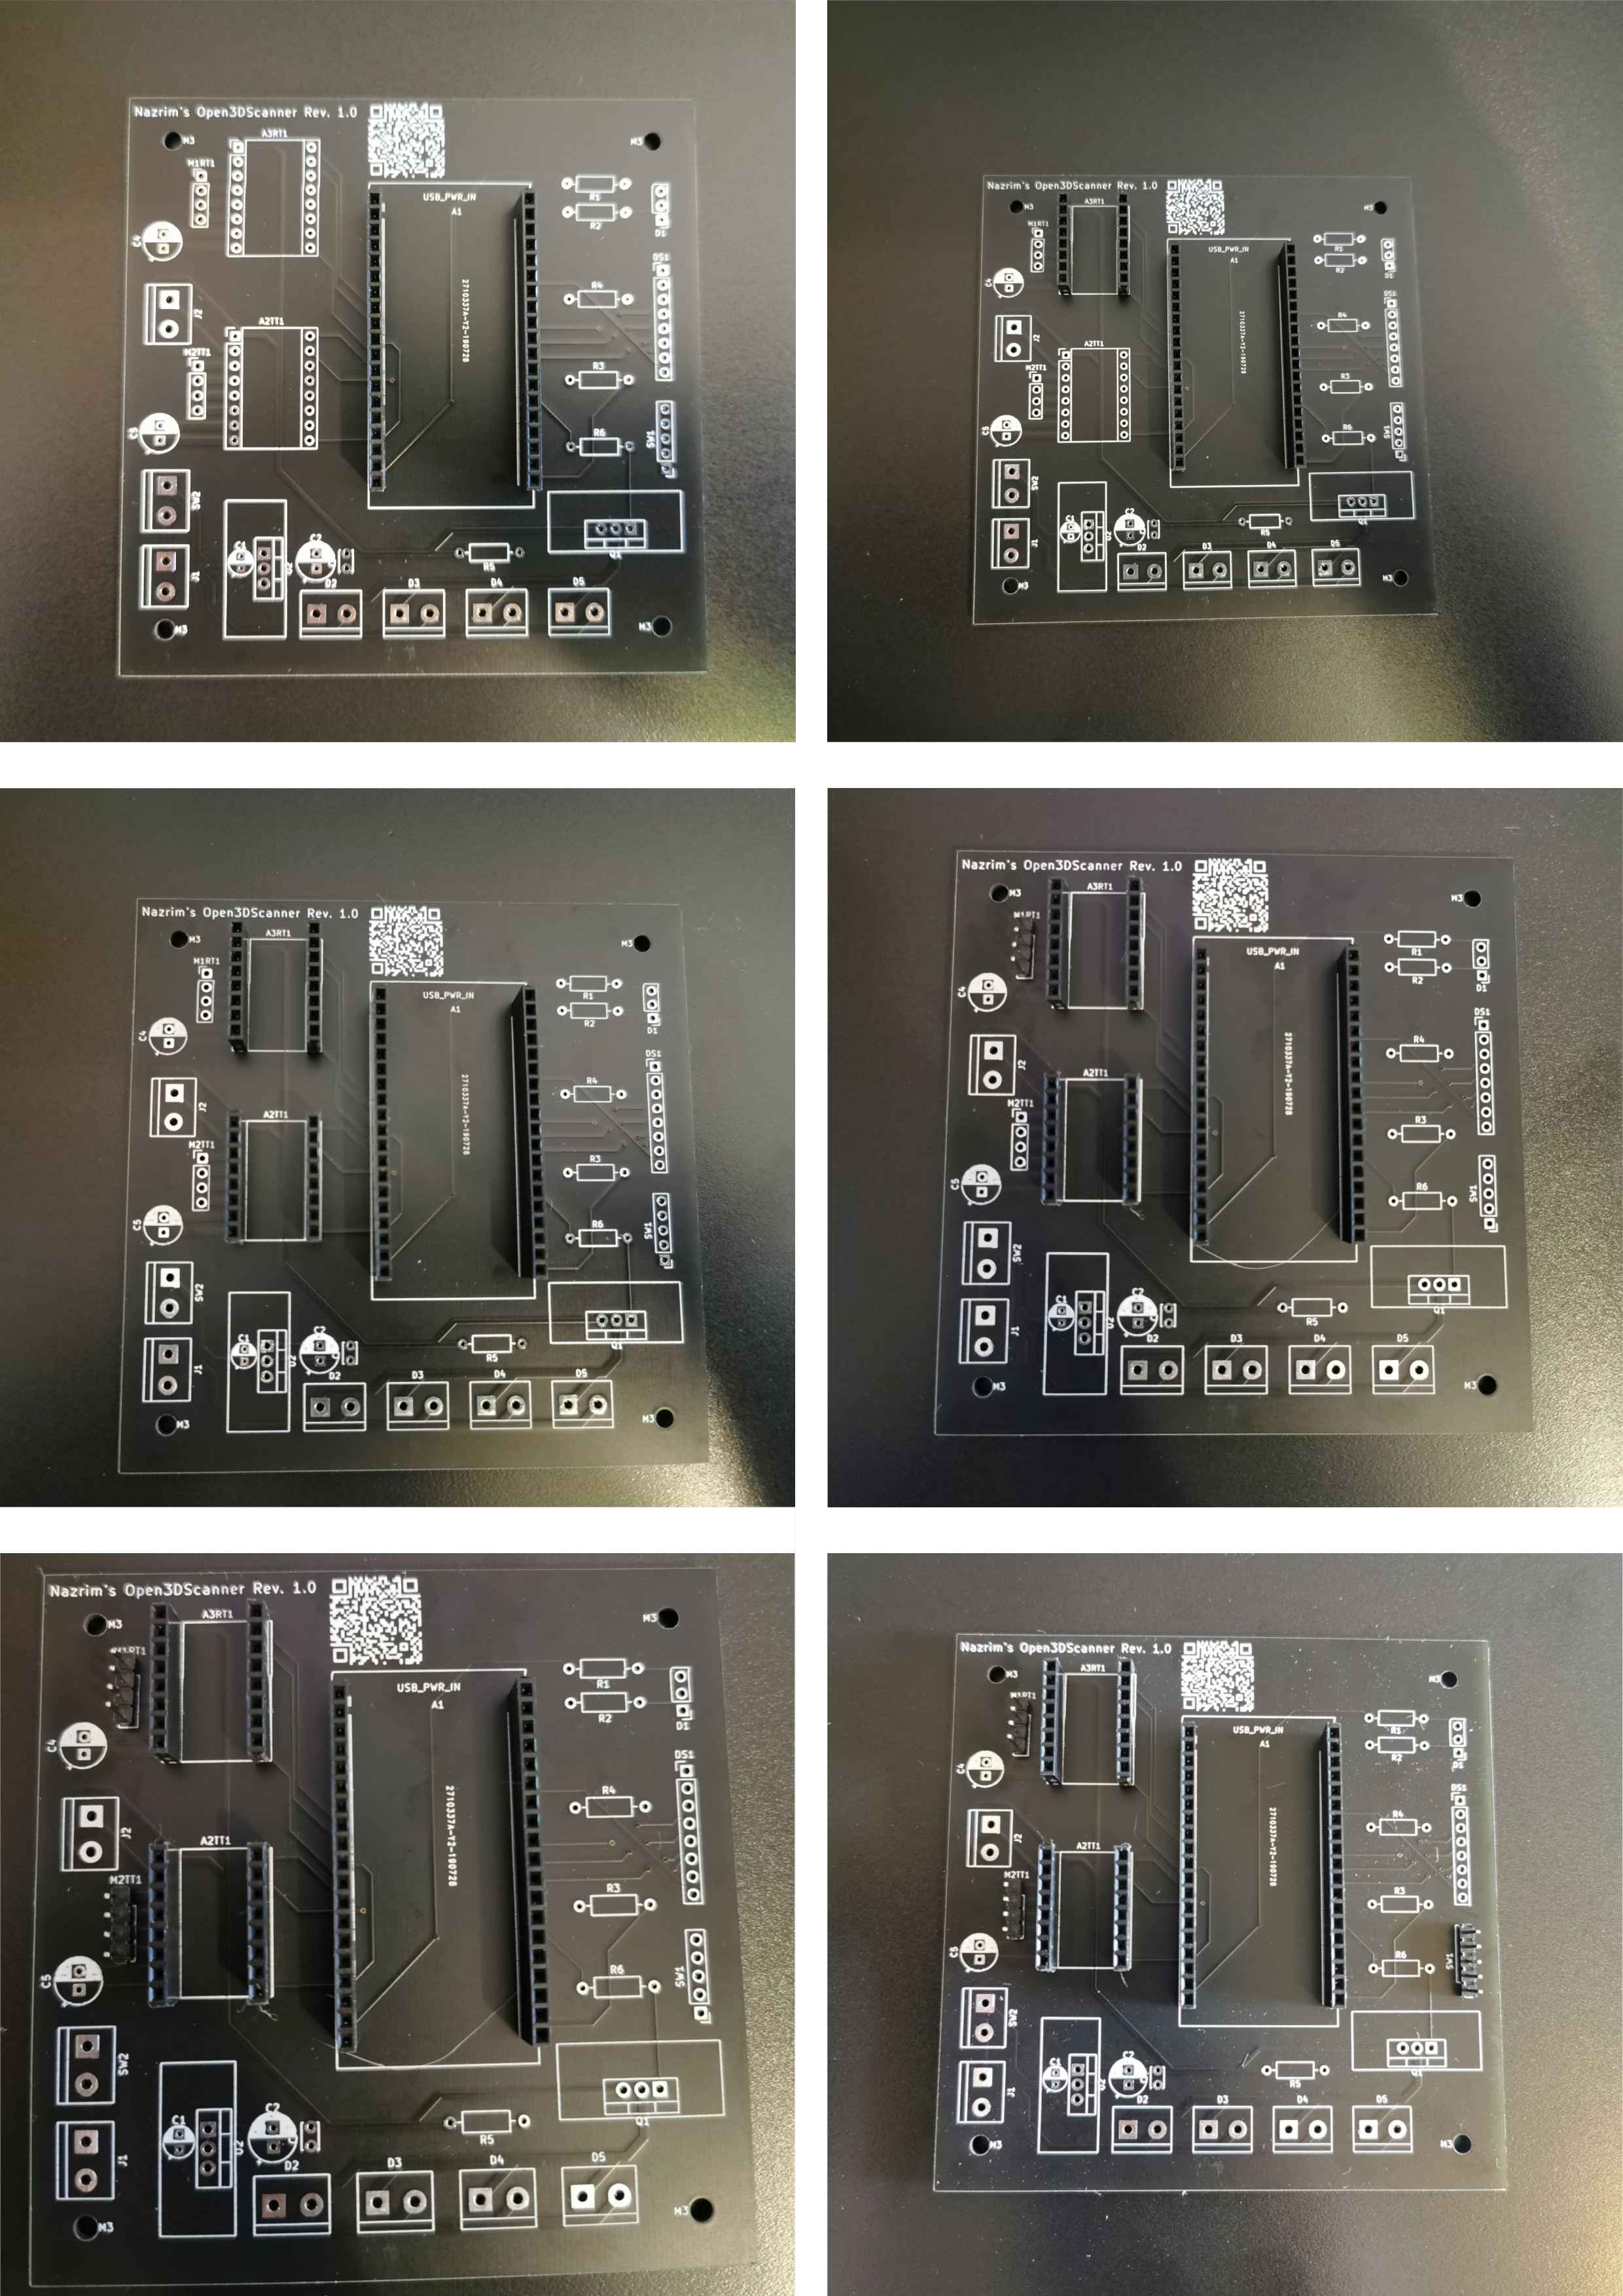
\includegraphics[width=\linewidth]{images/PcbSeries1.jpg}%
		\caption{Steps \numrange[text-rm=\lightBoldFont]{1}{6} of PCB assembly}%
	\end{centered}%
\end{figure}%

\begin{figure}[ht!]%
	\begin{centered}%
		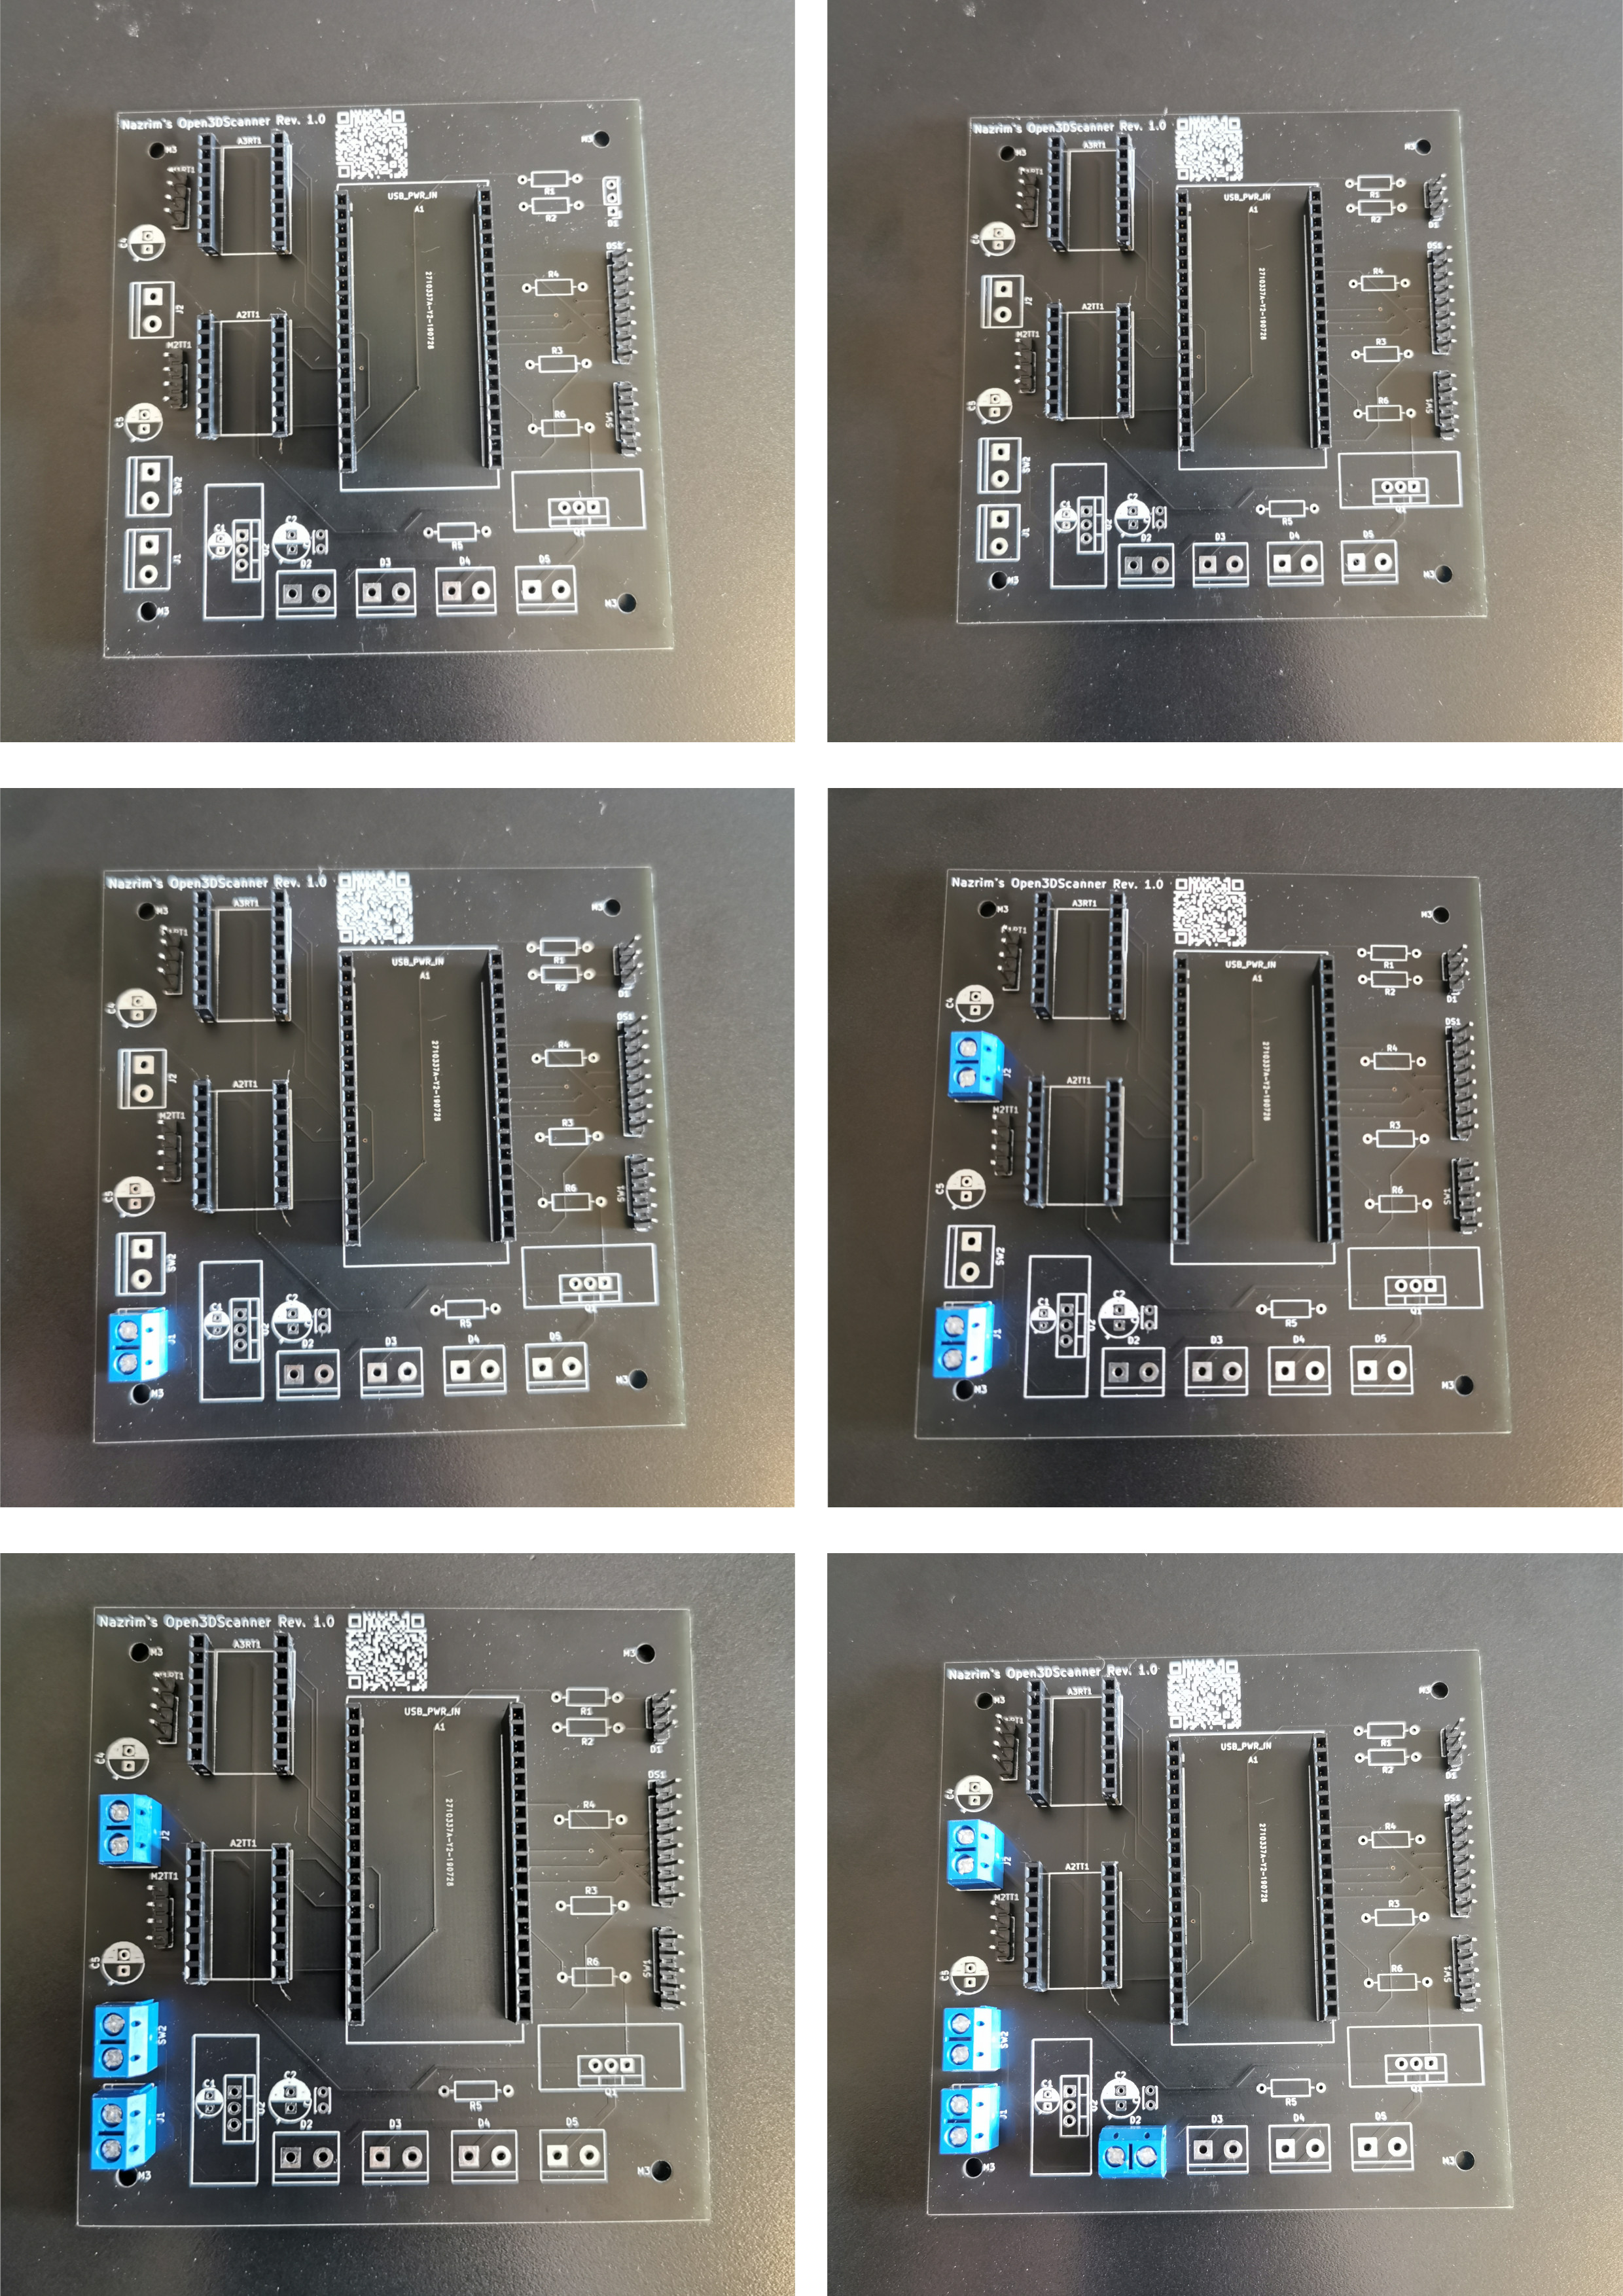
\includegraphics[width=\linewidth]{images/PcbSeries2.jpg}%
		\caption{Steps \numrange[text-rm=\lightBoldFont]{7}{12} of PCB assembly}%
	\end{centered}%
\end{figure}%

\begin{figure}[ht!]%
	\begin{centered}%
		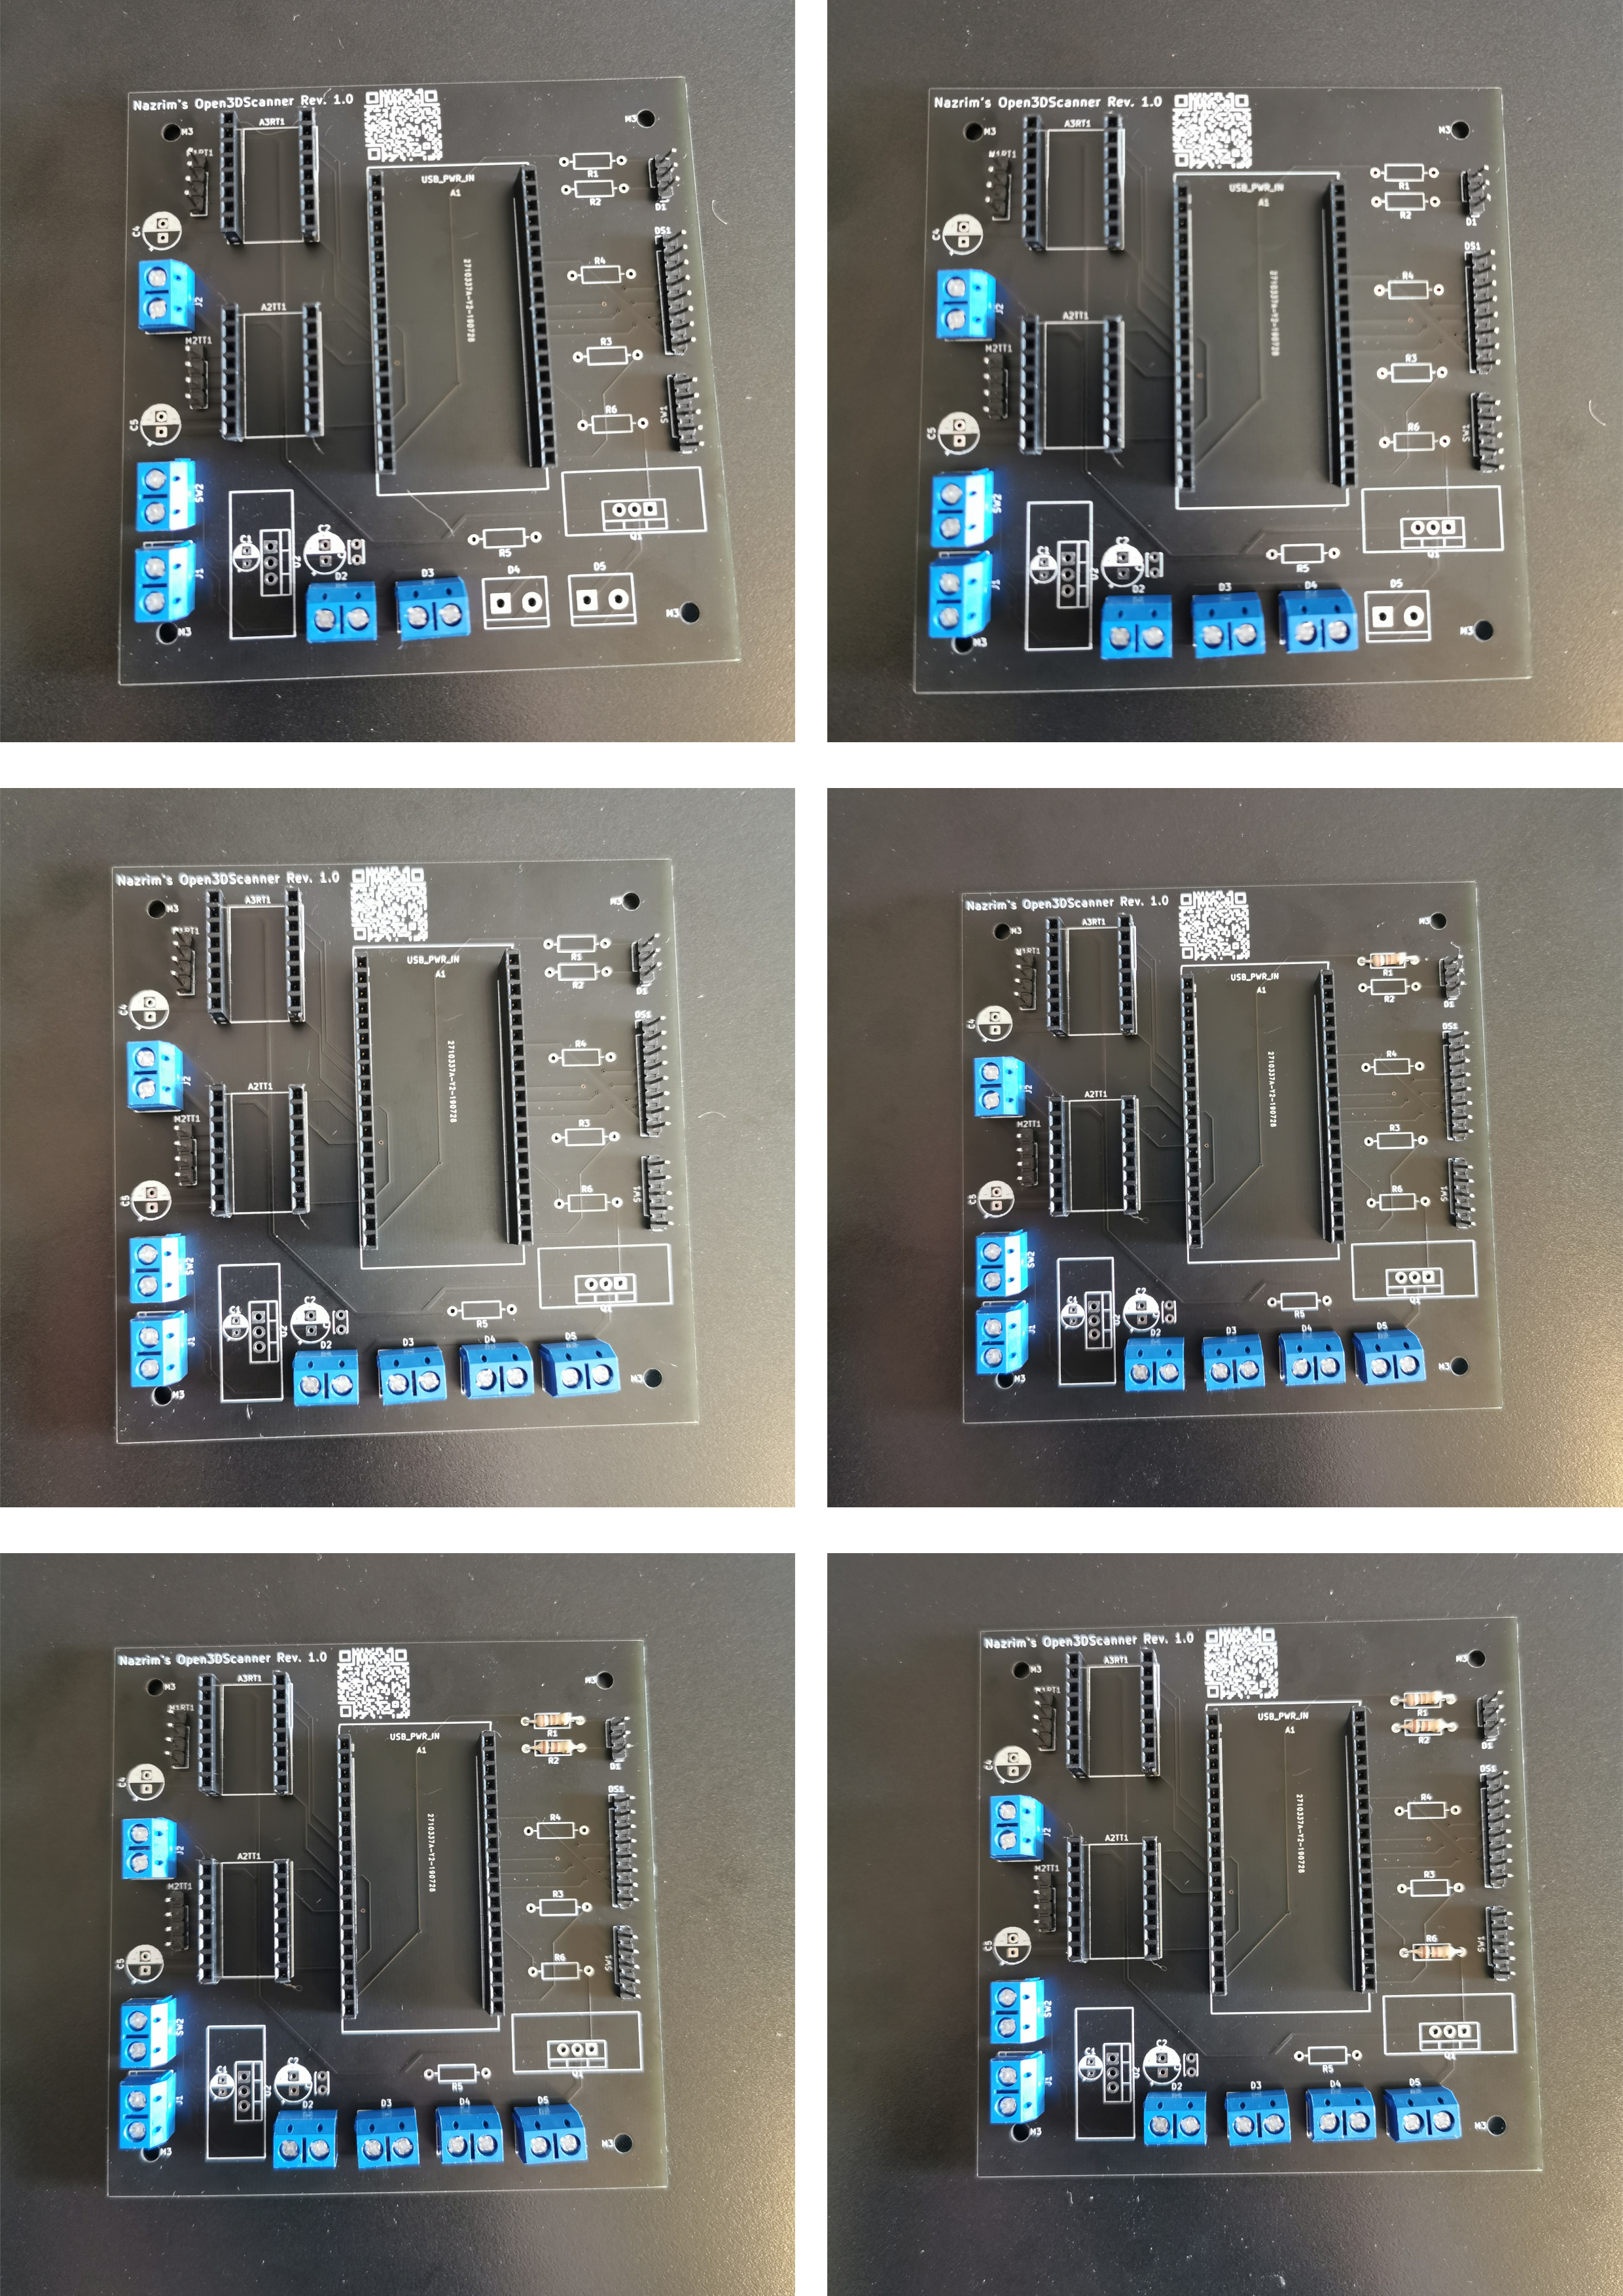
\includegraphics[width=\linewidth]{images/PcbSeries3.jpg}%
		\caption{Steps \numrange[text-rm=\lightBoldFont]{13}{18} of PCB assembly}%
	\end{centered}%
\end{figure}%

\begin{figure}[ht!]%
	\begin{centered}%
		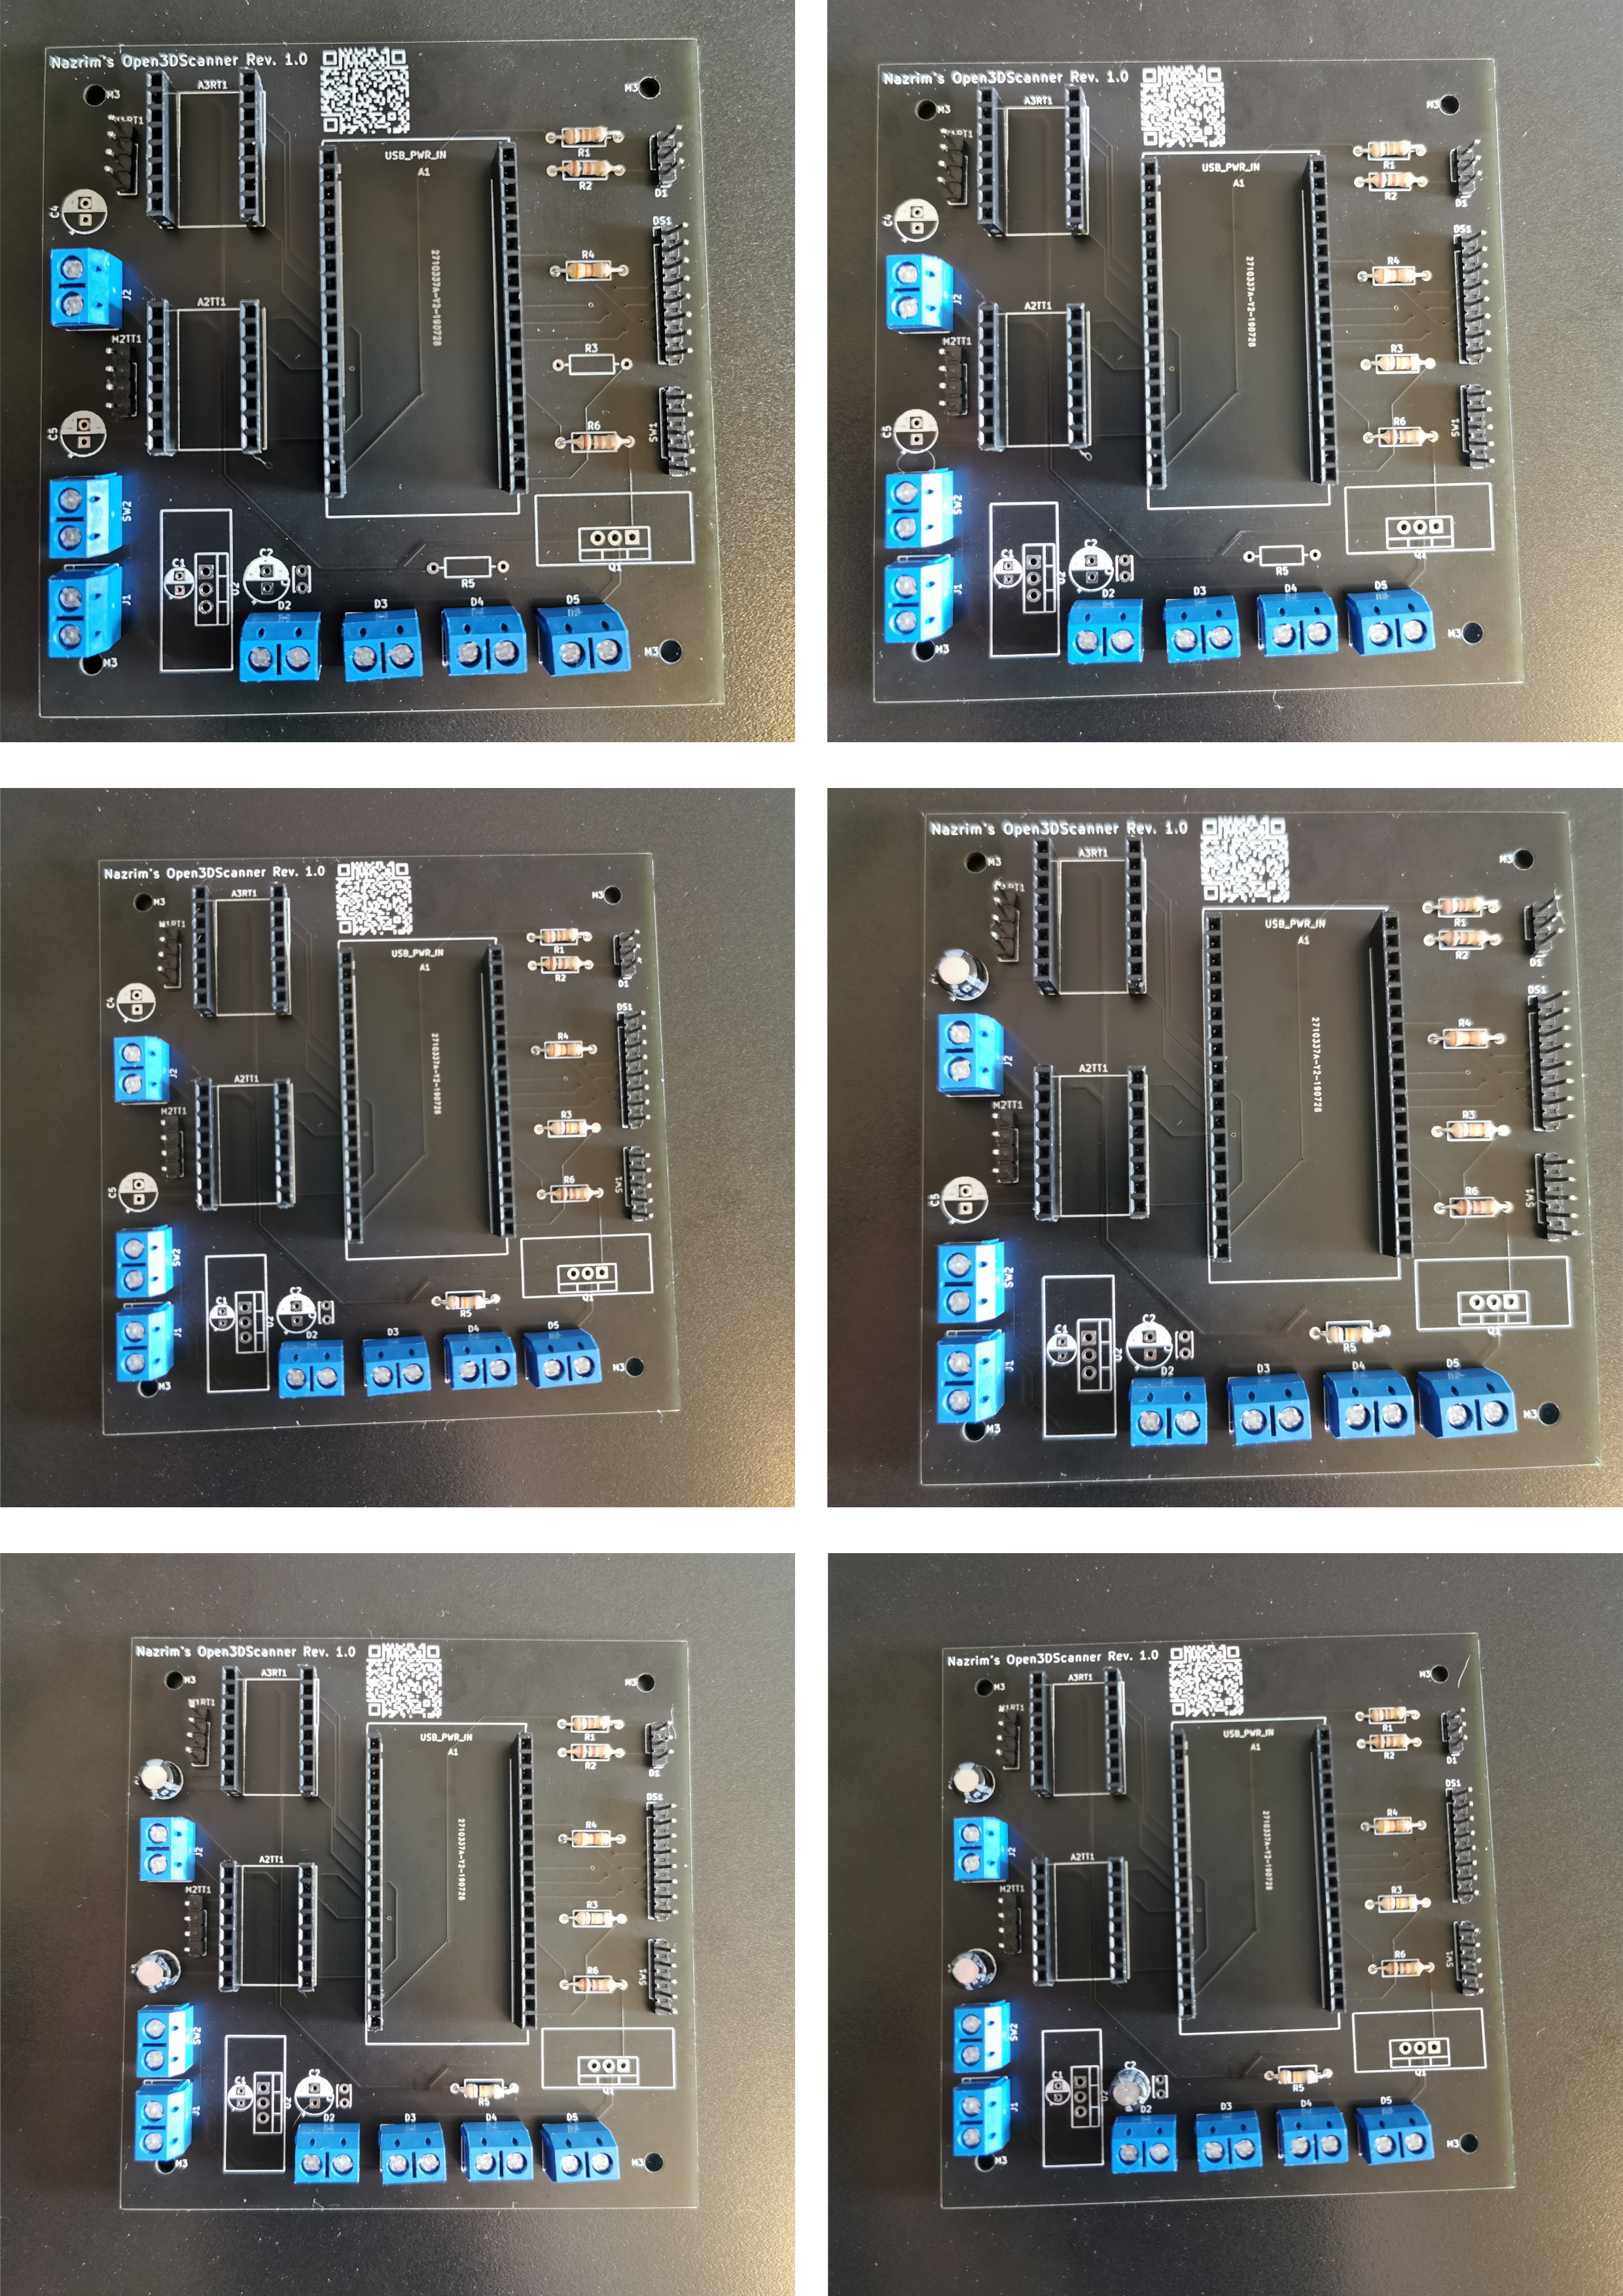
\includegraphics[width=\linewidth]{images/PcbSeries4.jpg}%
		\caption{Steps \numrange[text-rm=\lightBoldFont]{19}{24} of PCB assembly}%
	\end{centered}%
\end{figure}%

\begin{figure}[ht!]%
	\begin{centered}%
		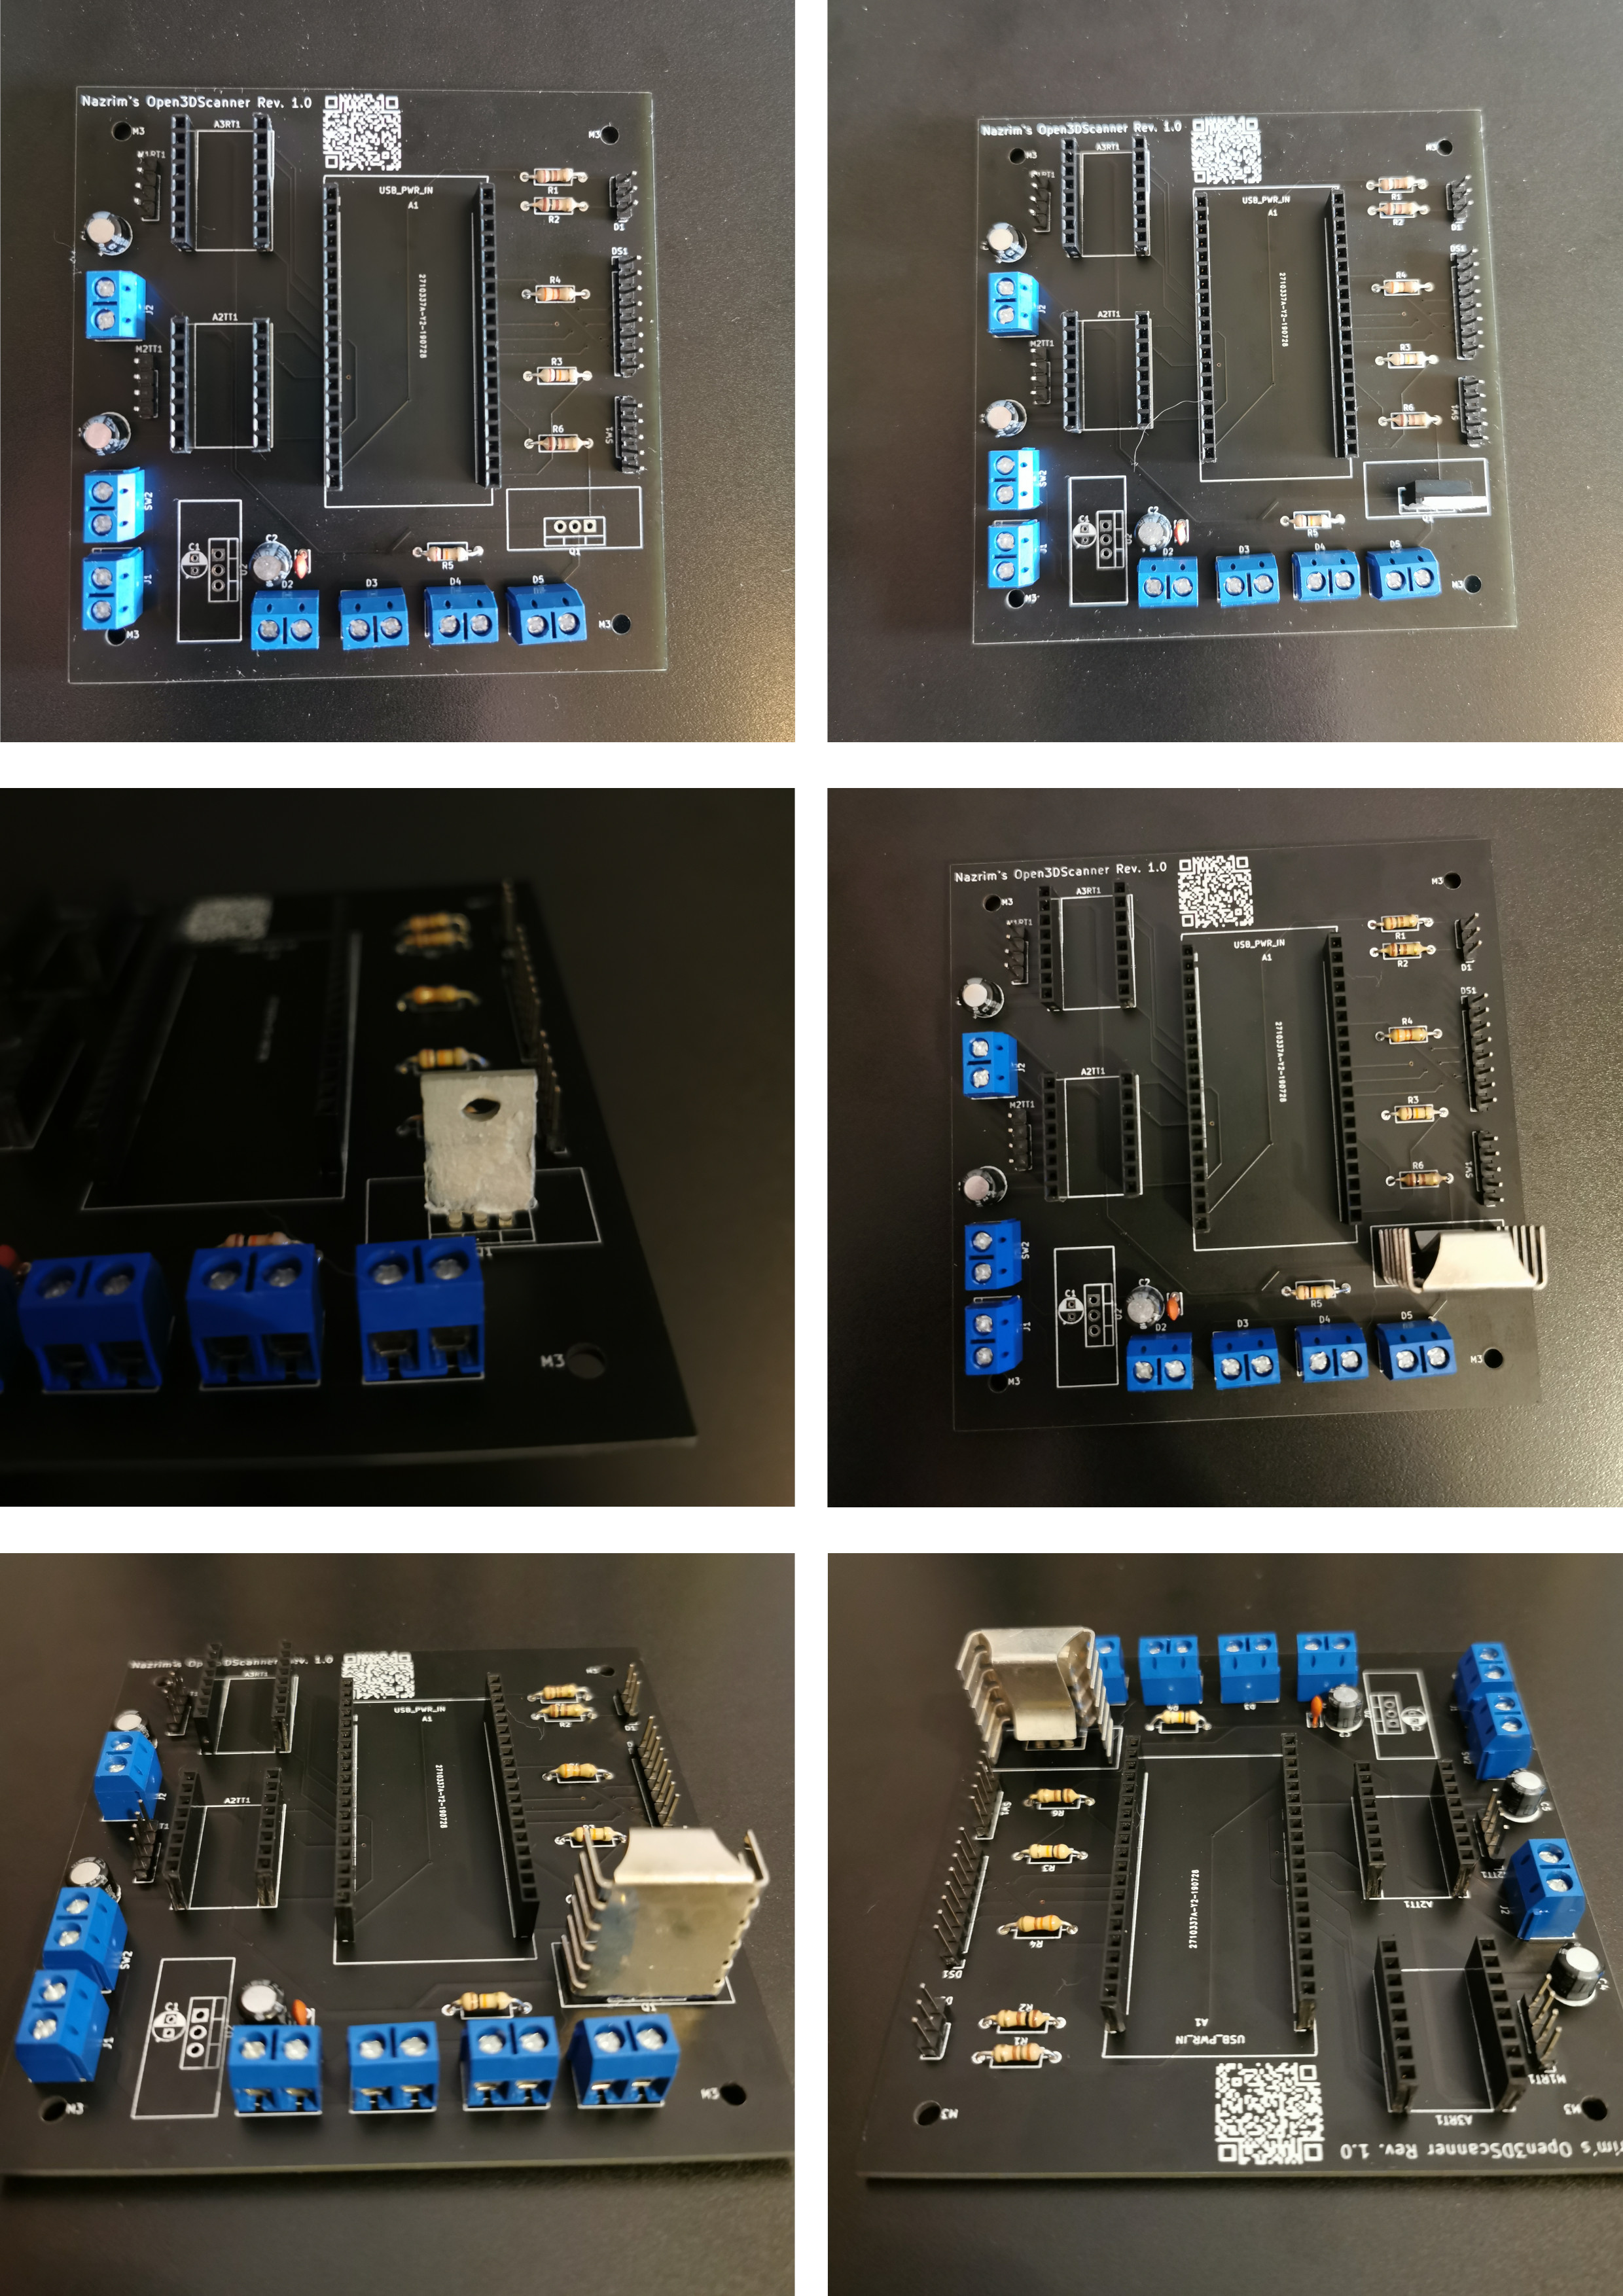
\includegraphics[width=\linewidth]{images/PcbSeries5.jpg}%
		\caption{Steps \numrange[text-rm=\lightBoldFont]{25}{30} of PCB assembly}%
	\end{centered}%
\end{figure}%

\begin{figure}[ht!]%
	\begin{centered}%
		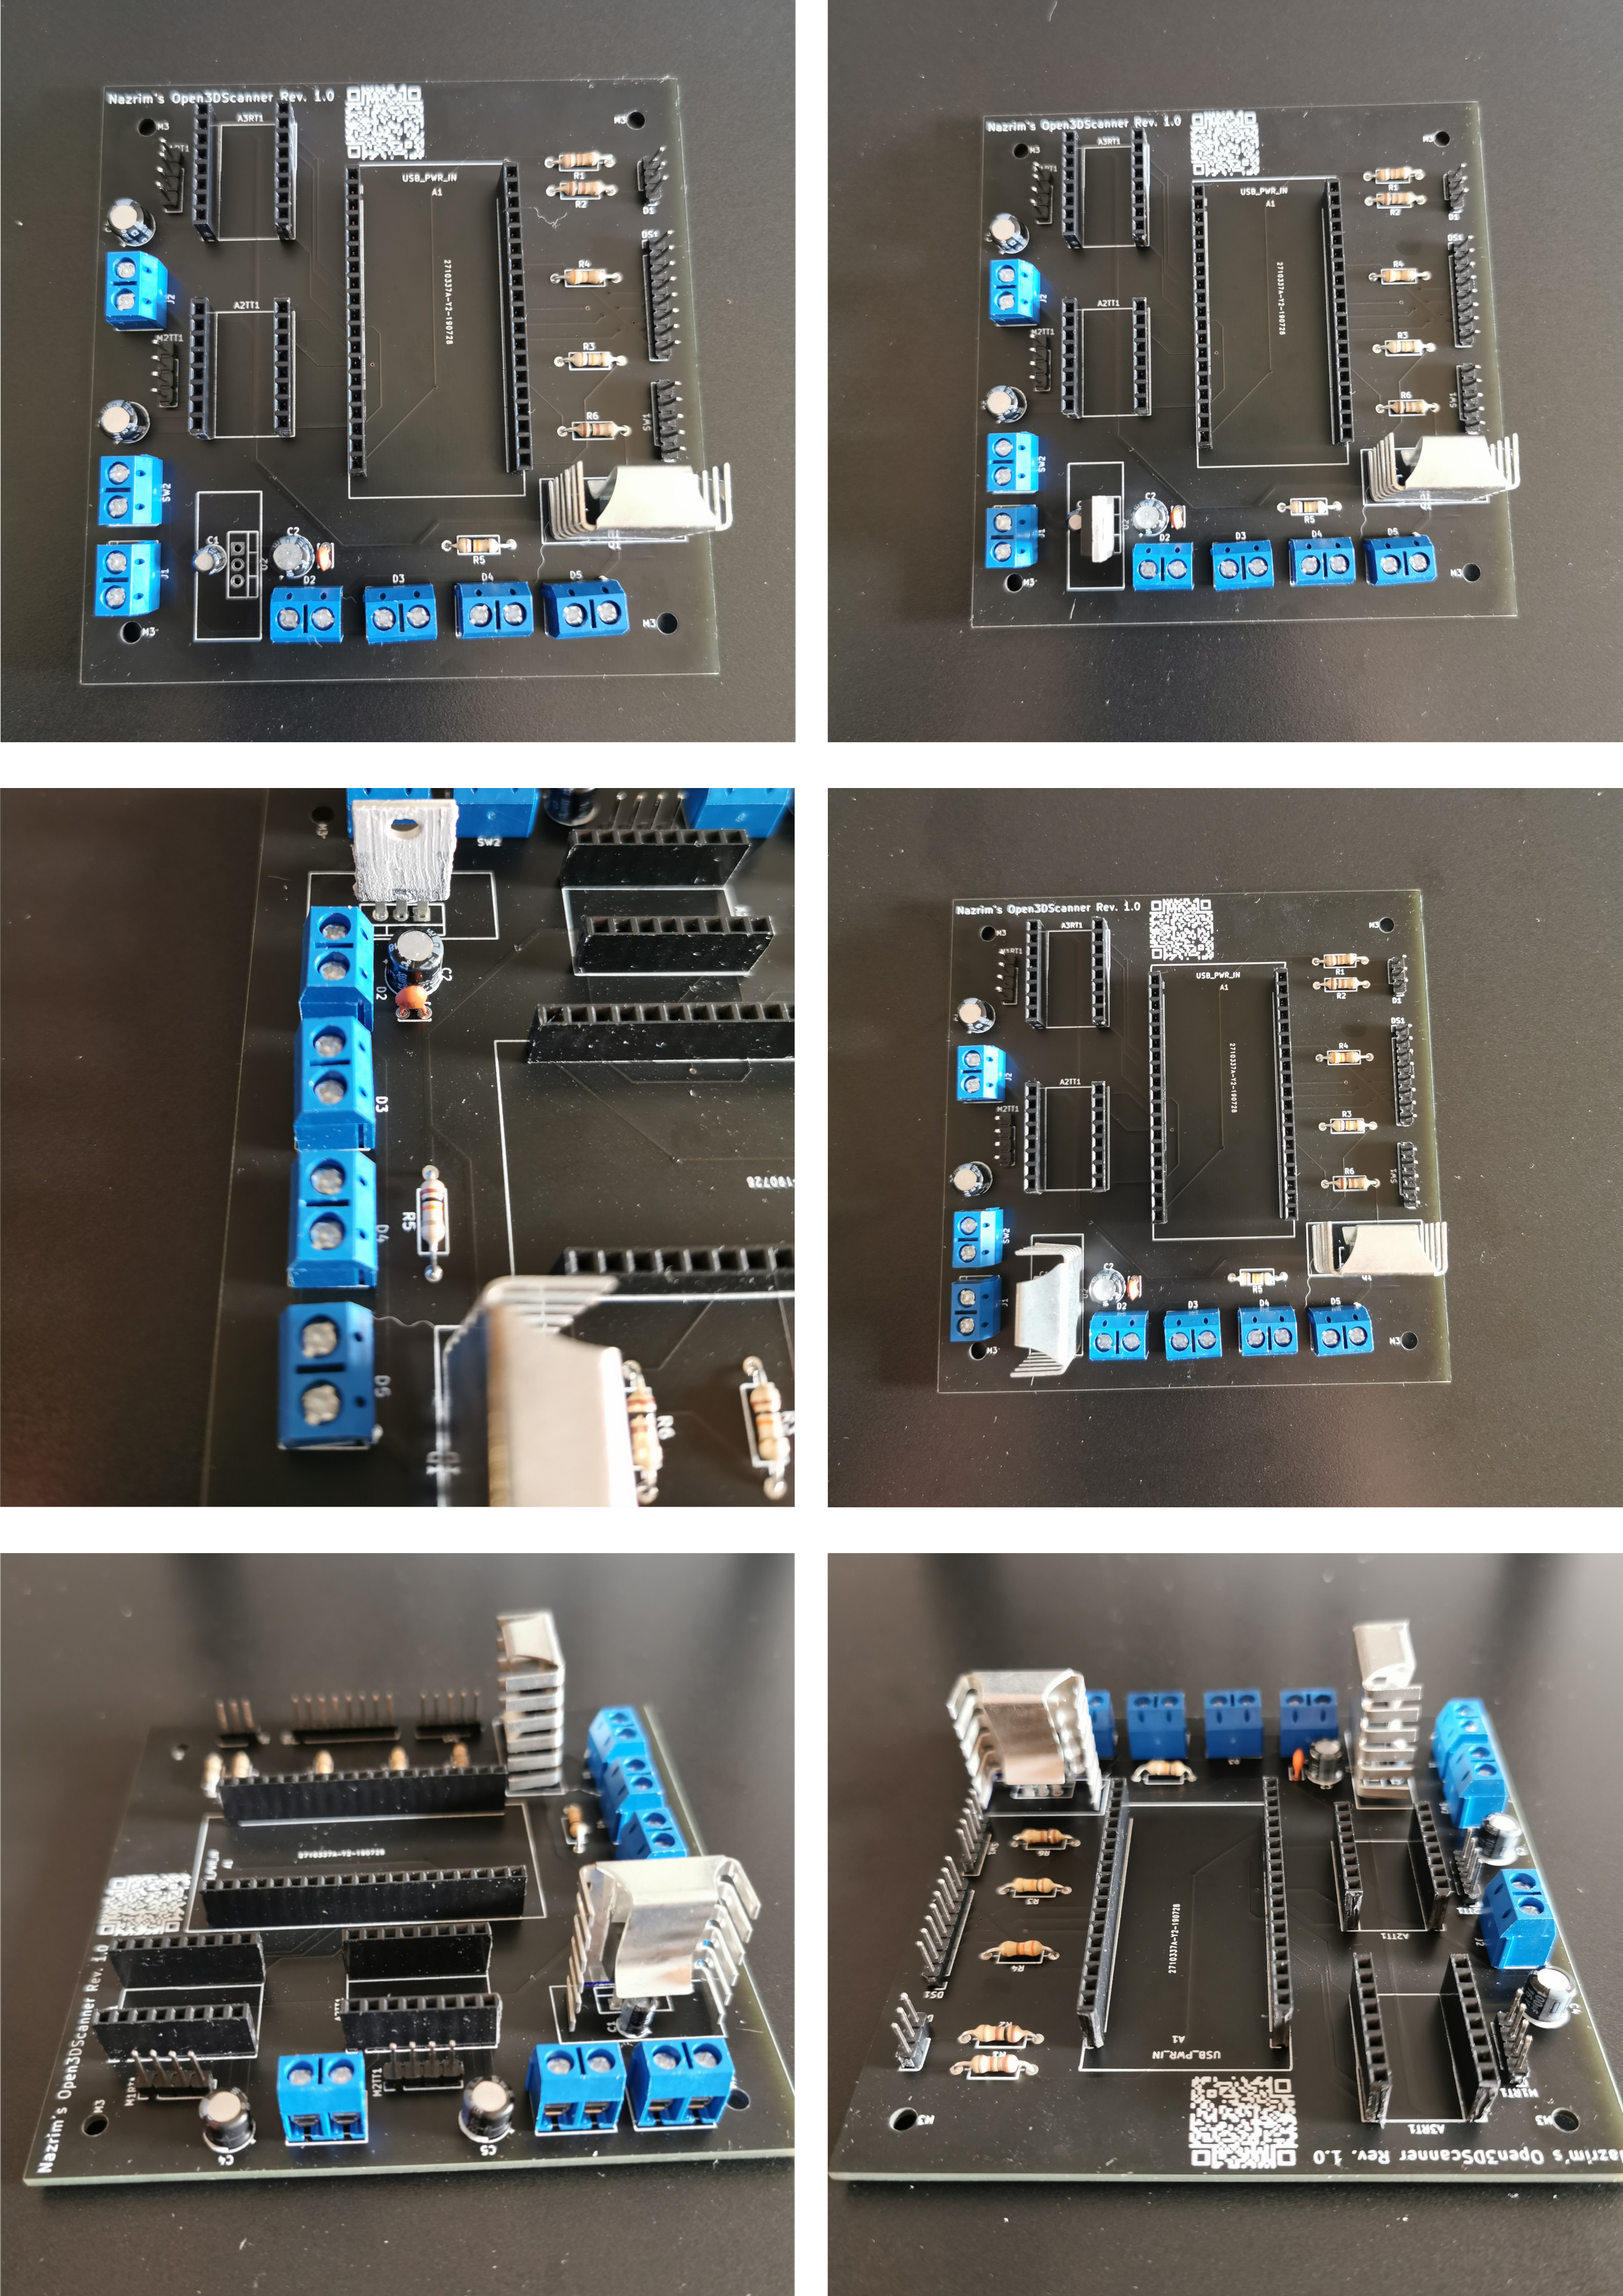
\includegraphics[width=\linewidth]{images/PcbSeries6.jpg}%
		\caption{Steps \numrange[text-rm=\lightBoldFont]{31}{36} of PCB assembly}%
	\end{centered}%
\end{figure}%

\begin{figure}[ht!]%
	\begin{centered}%
		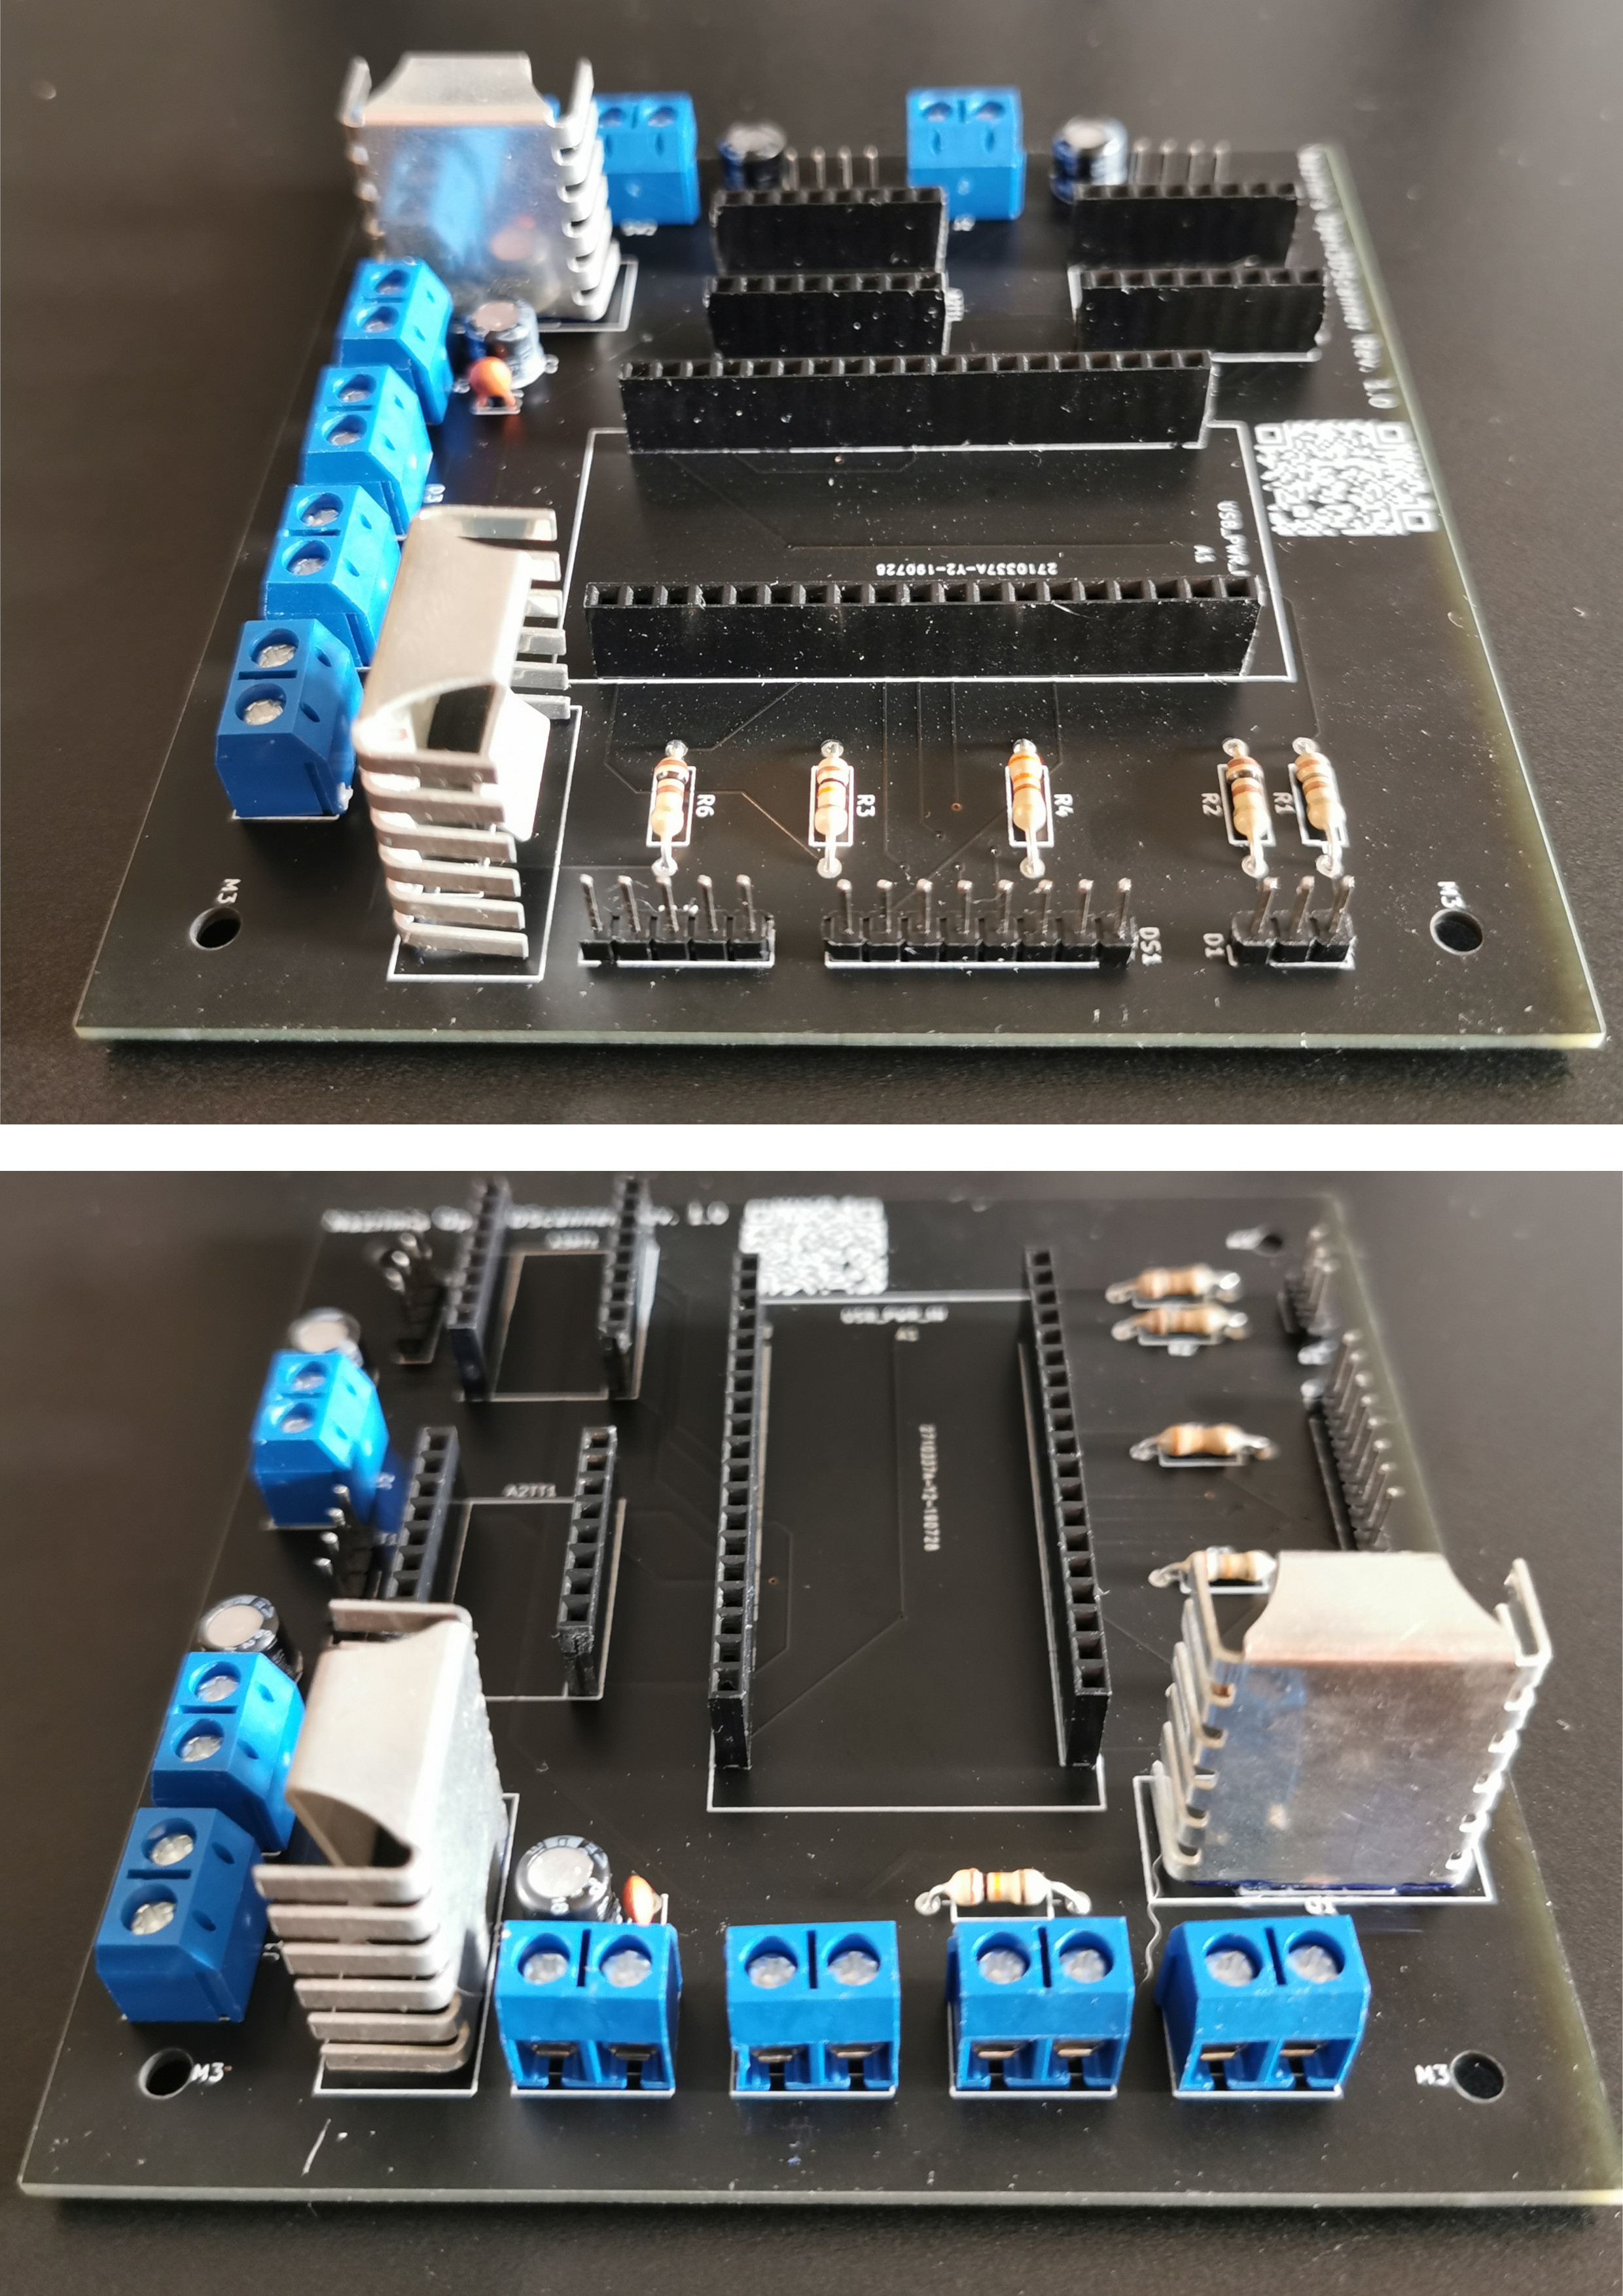
\includegraphics[width=\linewidth]{images/PcbSeries7.jpg}%
		\caption{Steps \numrange[text-rm=\lightBoldFont]{37}{38} of PCB assembly}%
	\end{centered}%
\end{figure}%